\chapter*{外文文献翻译}
{\centering
\begin{minipage}{\linewidth}
	\centering
	\xiaosan
	\bfseries
	《多人区域姿态估计网络》\\ 
	RMPE: Regional multi-person pose estimation
\end{minipage}
}
\label{cha:engtrans}
\section*{摘要}
在开放场景多人姿态估计是一个非常有挑战的任务。虽然现有的人体检测器已经展现出较好的效果,但是在一些困难场景下检测和识别误差中仍然无法避免。这些误差会导致在多人姿态检测系统系统在单人姿态估计网络阶段产生失误,尤其是一些非常依赖人体检测结果的方法。在本文中,我们提出了一种全新的区域多人姿态估计架构,用于改善人体检测器中可能出现的误差。我们的框架由三部分组成:对称空间变换网络,参数化姿态极大值抑制,以及姿态引导的目标框引导生成器。我们的方法可以应对不准确的检测框,并产生冗余的检测结果,让本方法在MPII数据集上达到76.7mAP的成绩。本文中的模型以及源码已经向公众开放。

\section*{引言}
人体姿态估计是一个计算机视觉领域中主要的挑战。在实践过程中,在开放环境中识别多人姿态要比从数字图像中恢复单人姿态更加有挑战性。近年的一些方法尝试通过两阶段框架,或者是一个基于部件的框架完成该任务。在两阶段的框架中,网络首先检测人体目标的边界框,之后对每一个边界框单独地回归姿态。而基于部件的框架首先检测所有的人体关键点,并根据检测到的人体关键点重新组装生成多个人体姿态。这两类框架都有各自的优点与缺点。对于两阶段框架而言,姿态估计结果高度依赖于人体检测框结果的质量。对于基于部件的框架而言,多人姿态估计结果可能会由于多个相互接近的人体而导致检测结果过于模糊。同时,由于基于部件的框架仅从底层考虑身体部件的结构,因此其难以全局地考量各个身体部位之间的关系。

我们的方法遵从两阶段框架。我们着眼于在不准确的目标检测框下检测精准的人体姿态。为了表现之前方法的缺陷,我们使用了现代检测器Faster R-CNN和用于但人姿态估计的堆叠沙漏网络进行了测试。如图1与图2中所示,一般两阶段的网络面临了一下两种缺陷:定位误差以及冗余检测。实际上,单人姿态估计网络是一个对目标检测结果容忍度很低的网络。即使在考虑交并比大于0.5为检出结果的条件下,单人姿态估计网络得到的单人姿态很有可能还是错误的。因为单人姿态估计网络针对于检测框生成姿态估计结果,一些冗余的检测结果就会得到冗余的姿态估计结果。

为了改善上述问题,本文提出了区域多人姿态估计框架。我们的框架改善了基于单人姿态估计网络的多人姿态估计算法。我们设计了附加在单人姿态估计网络后对称空间变换网络来从不精确的目标检测框中提取高质量的单人人体区域。在本文中,这些单人人体姿态估计网络都是以并行的方式排布在我那个罗中。同样为了消除检测冗余的问题,我们还引入了参数化姿态极大值抑制。我们的参数化姿态极大值抑制使用全新的姿态距离评价来给出姿态相似度,从而消除冗余的姿态估计结果。最后,我们设计了全新的姿态引导的人体检测框生成器来扩增训练样本。通过学习人体检测器对于不同姿态的输出分布,可以模仿检测器生成大量的训练样板。

我们区域多人姿态估计框架可以被迁移至不同的人体检测器与单人姿态估计算法中。我们在MPII数据集上进行训练并验证,并得到了76.7mAP的成绩。我们同时设计了效能实验来验证我们在框架中提出的不同部件对于网络性能的贡献。本文方法的模型与源代码现在已经向公众开放,用来支撑本文得出的可复现的实验结果。

\section*{区域多人姿态估计}
本文提出的区域多人姿态估计的框架如图3所示。从人体检测器中得到的人体检测框被送入对称空间变换网络+单人姿态估计网络中,然后自动生成姿态检测框。这些被生成的检测框被参数化姿态极大值抑制精简,用来框住提取到的人体姿态。在训练过程中,我们使用并行化的单人姿态估计网络来在避免陷入局部最优的同时促进对称空间变换网络对于检测结果的性能强化。为了扩增现有的训练样本,我们设计了姿态引导的检测框生成器。在接下来的几节中,我们主要论述框架中三个模块的设计思路。
\subsection*{对称空间变换网络与并行的单人姿态估计网络}
由人体检测器提供的人体检测框并不是很适合单人姿态估计网络。这是因为单人姿态网络在训练时是仅使用单人图像的因此它们对于一些定位误差十分敏感。一些对检测框的细微调整或者是裁剪可以有效地改善单人姿态估计网络的性能。本文中的对称空间变化网络以及并行单人姿态估计网络的提出旨在提高单人姿态估计网络在不完美人体检测框下的性能。对称空间变换网络与并行的单人姿态估计网络结构如图4所示。

\textbf{空间变换网络与逆空间变换网络} 空间变换网络在自动选择兴趣区域时体现出了极好的性能。在本文中,我们使用空间变换网络来提取高质量的显著人体检测框。从数学上来讲,空间变换网络可以被描述为:
\begin{equation}
\label{rmpe:1}
\begin{pmatrix}
x_i^s \\
y_i^s
\end{pmatrix}
= 
\begin{bmatrix}
\theta_1 & \theta_2 & \theta_3
\end{bmatrix}
\begin{pmatrix}
x_i^t \\
y_i^t \\
1
\end{pmatrix}
\end{equation}
在公式\eqref{rmpe:1}中,$\theta_1$,$\theta_2$和$\theta_3$是一个在$\mathbb{R}^2$中的向量。$\{x_i^s, y_i^s\}$和$\{x_i^t,y_i^t\}$分别是空间变换前后的坐标。在单人姿态网络后,姿态结果会被映射到原始的图像中。很自然地,在这之后需要一个逆空间变换网络来将估计到的人体姿态重新映射到原始图像的坐标系中。这里逆空间变换网络计算$\gamma$来对坐标进行逆变换。
\begin{equation}
\label{rmpe:2}
\begin{pmatrix}
x_i^t \\
y_i^t
\end{pmatrix}
= 
\begin{bmatrix}
\gamma_1 & \gamma_2 & \gamma_3
\end{bmatrix}
\begin{pmatrix}
x_i^ts\\
y_i^s\\
1
\end{pmatrix}
\end{equation}
由于逆空间变换网络是一个空间变换网络的逆过程,因此我们可以得到:
\begin{equation}
\label{rmpe:3}
\begin{bmatrix}
\gamma_1 & \gamma_2
\end{bmatrix}
=
\begin{bmatrix}
\theta_1 & \theta_2
\end{bmatrix}^{-1}
\end{equation}

\begin{equation}
\label{rmpe:4}
\gamma_3 = -1 \times 
\begin{bmatrix}
\gamma_1 & \gamma_2
\end{bmatrix}
\theta_3
\end{equation}

为了能够让梯度通过逆空间变换网络回传,$\frac{\partial J(W, b)}{\partial \theta}$对$\theta_1$与$\theta_2$的偏导可以被求解为:
\begin{equation}
\label{rmpe:5}
\frac{\partial J(W, b)}{\partial \begin{bmatrix} \theta_1 & \theta_2\end{bmatrix}} = 
\frac{\partial J(W, b)}{\partial \begin{bmatrix} \gamma_1 & \gamma_2\end{bmatrix}} \times \frac{\partial \begin{bmatrix} \theta_1 & \theta_2\end{bmatrix}}{\partial \begin{bmatrix} \gamma_1 & \gamma_2\end{bmatrix}} + \frac{\partial J(W, b)}{\partial \gamma_3} \times \frac{\partial \gamma_3}{\partial \begin{bmatrix} \gamma_1 & \gamma_2\end{bmatrix}} \times  \frac{\partial \begin{bmatrix} \theta_1 & \theta_2\end{bmatrix}}{\partial \begin{bmatrix} \gamma_1 & \gamma_2\end{bmatrix}}
\end{equation}

同样地,$\frac{\partial J(W, b)}{\partial \theta}$对$\theta_3$的偏导可以被求解为:
\begin{equation}
\label{rmpe:6}
\frac{\partial J(W,b)}{\partial \theta_3} = \frac{\partial J(W,b)}{\partial \gamma_3} \times \frac{\partial \gamma_3}{\partial \theta_3}
\end{equation}
$\frac{\partial \begin{bmatrix} \theta_1 & \theta_2\end{bmatrix}}{\partial \begin{bmatrix} \gamma_1 & \gamma_2\end{bmatrix}}$与$\frac{\partial \gamma_3}{\partial \theta_3}$可以被分别求解为公式\eqref{rmpe:3}与公式\eqref{rmpe:4}。

在提取完高质量的人体检测框之后,我们可以整合现有的单人姿态估计网络来提取高精度的多人人体姿态。在我们的训练过程中,对称空间变换网络在后调整步骤中与单人姿态网络联合训练。

\textbf{并行单人姿态提取网络} 为了之后更好地帮助空间变换网络提取更好的显著人体区域,我们在训练阶段添加了并行单人姿态提取网络。这个分支与原有的单人姿态估计网络共享同一个空间变换网络,但是逆空间变换网络被省略了。在该分支中所有的人体姿态都被放置至中央。确切地讲,单人姿态网络分支的输出直接与真值标签做比较。我们在训练过程中冻结了所有在并行单人姿态估计网络中的参数。所有由该分支产生的误差都被累加至了空间变换网络中。如果被空间变换网络提取的姿态并不是中心对齐的,那么并行分支会将错误好回传以修正空间变换网络产生的误差。如此一来,我们可以帮助空间变换网络去关注争取的区域,并提取高质量的人体显著检测框。在验证过程中,并行的单人姿态估计网络被取消。该部分的有效性在之后的实验中将被证明。

\textbf{讨论} 并行的单人姿态估计网络是可以被认为是一个在训练过程中对于空间变换网络的正则项。它能够帮助网络避免过差的无法让网络定位姿态中心的区域最优解。由于逆空间变换网络会让网络生成更少的错误,因此其陷入局部最优的可能性就可能会有所提高。这些错误对于训练空间变化网络而言至关重要。通过引入并行单人姿态提取网络,空间变换网络会被并行分支促进逐渐将输出靠近姿态估计结果的中心。

从直觉上来讲,用一个中央对齐的姿态回归损失函数替换一个并行的单人姿态提取网络是一个更加直接的办法。但是,这种方法会降低我们系统的表现。尽管空间变换网络可以部分地变换输入,然而将人完美地重新放置在真值所出现的位置仍然是不可能的。预测值与真值之间的坐标差距会大大损害我们学习姿态估计的过程。这会导致我们主单人姿态估计网络性能表现的下降。所以,为了确保空间变换网络与单人姿态估计网络能够共同相互促进,一个固定参数的并行单人姿态估计网络是不可替换的。并行的单人姿态估计网络总会对为中央对齐的姿态估计结果产生巨大的误差,因而会促进空间变换网络在不损害主分支性能的条件下生成中央对齐的人体检测框结果。

\subsection*{参数化姿态极大值抑制}
人体检测器会不可避免地生成冗余检测结果。这会让姿态估计网络生成冗余的姿态估计结果。因此,姿态极大值抑制对于消除冗余是必须的。近年方法中提出的极大值抑制都会遇到效率或准确度上的问题。在本文中,我们提出了参数化的姿态极大值抑制来解决这些问题。与之前章节中所描述相似,带有$m$个躯干的姿态信息$P_i$可以被表示为$\{<k_i^1, c_i^1>, ...,<k_i^m, c_i^m>\}$,其中$k_i^j$与$c_i^j$分别表示第$j$个关键点的坐标与置信度。

\textbf{极大值抑制策略} 我们重新定义姿态极大值抑制如下:首先,置信度极大值位置的关键点信息被筹集起来,然后其周围的是关键带你位置就会被\textit{消除原则}所消除。这个过程被重复数次用于消除冗余的姿态估计结果,并得到最终独一无二的姿态估计信息。

\textbf{优化} 根据给定检测到的冗余姿态,在消除原则中的四个参数会被被优化以在验证数据集中达成最高的mAP。因为在四维空间里穷举查找一个最优值是不可能得,所以我们每次优化时固定两个参数的同时优化另两个参数。一旦收敛,参数将被固定并应用于测试阶段。

\subsection*{姿态引导的检测框生成器}
\textbf{数据增强} 对于两阶段的多人姿态估计方法,合适的数据增强方法能够让对称空间变换网络+单人姿态估计网络模块适应人体检测器生成人体检测框的“不完美”。如果不做扩增,那么模块可能没有办法在测试阶段适应人体检测器。最初始的方法是直接使用由人体检测器生成的检测框去训练网络。然而,人体检测器只能给出每个人的检测框。通过使用一个检测框生成器可以让网络在训练时增加检测框的数量。由于我们已经拥有了每个人的检测框和姿态信息的真值,那么我们就可以根据人体检测器生成检测框的分布生成大量的训练检测框。通过应用这个技术,我们便有可能在之后验证中增强我们系统的性能。

\textbf{数据整理} 我们发现检测框相对真值偏移量的分布和不同的姿态有相关性。确切地说,存在一个$P(\delta B|P)$,使得$\delta B$是真值与预测值之间检测框坐标的偏差值,同时$P$是一个目标的人体姿态信息。如果我们能够对这个概率分布进行建模,那么我们就可以像人体检测器一样生成训练用的检测框了。

\textbf{实现} 由于人体姿态信息多种多样,直接学习$P(\delta B|P)$的分布是一件较为困难的事情。所以相反地,我们尝试学习$P(\delta B|atom(P))$,其中$atom(P)$代表一个代表$P$的原子姿态。我们遵从Andriluka等人的工作去学习原子姿态。为了从标注数据中推到原子姿态,我们首先对齐多有的躯干,让他们的躯干长度拥有相同的长度。之后我们使用K-均值算法聚类对齐后的姿态,同时计算我们得到的原子姿态距离每个聚类中心的距离。现在对于每一个符合原子姿态$a$的人体目标,我们都会计算其检测结果与真值检测框的偏移量。这些偏移量被真值检测框的边长所归一化。如此一来,这些偏移量就会构建起一个频率分布,因此我们可以使用高斯混合模型去拟合我们的数据。对于不同的原子姿态,我们都有不同的高斯混合模型参数去描述。我们将部分分布可视化并对将对应的聚类结果在图5中展示。

\textbf{检测框生成} 再对称空间变换网络与单人姿态估计网络的训练过程中,对于每一个标注的训练用姿态信息,我们首先会去浏览它们对应的原子姿态$\alpha$。然后我们根据$P(\delta B|a)$生成对应的加性偏移量,以构造扩增的训练检测框。

\section*{实验}
本文提出的方法使用两个标准数据集:MPII与COCO 2016 Challenge数据集进行量化评测。

\subsection*{测试数据集}
\textbf{MPII 多人数据集} MPII多人数据集包括3844组包含多人的图像和1758组测试用多人图像。在验证与训练数据集中,都同时有出现遮挡和交叠的情况发生。同时,它拥有多于28000张的用于训练单人姿态估计网络的训练数据集。我们首先使用所有的训练数据集和90\%的多人数据集来调整单人姿态估计网络,留下10\%的多人数据集作为验证数据。

\textbf{MSCOCO Keypoints Challenge} 我们同样使用我们的方法在MSCOCO Keypoints Challenge上进行了评测。这个数据集需要在无法控制的情况下给出关键点定位结果。它包含了105698张训练数据和大概80000张测试数据。训练数据集囊括了至少一百万个标注的关键点。数据集的测试集被分成了4等分:测试挑战,测试验证,测试标准和测试保留。

\subsection*{验证细节}
本文中我们使用了基于VGG的SSD-512作为我们的人体检测器,因为它能够又快又准地给出目标位置。为了保证我们整个人体区域都被检测到,检测框的长宽被扩张了30\%。我们使用了堆叠沙漏网络作为我们单人姿态估计网络因为其卓越的性能。对于空间变换网络,我们使用了ResNet-18作为我们的定位网络 。考虑到内存的效率,我们使用了4阶段的堆叠沙漏网络作为我们的并行单人姿态估计网络。

\subsection*{结果}
\textbf{MPII数据集结果} 我们在MPII多人数据集上进行了性能评价。在全部验证集上的验证结果如表1所示。值得注意的是,我们在一些困难的关键点,比如手腕,手肘,脚踝和膝盖等部位达成了72mAP的成绩,比现有最好方法高出3.3mAP。我们模型还在手腕的最终结果达到了70.4mAP,同时在膝盖检测达成了73mAP的成绩。我们将一些结果的可视化放在了图6中。这些结果反应我们的模型能够准确的预测多人图像中的姿态信息。更多的结果请参阅补充材料。

\textbf{在COCO数据集上的结果} 我们在COCO训练和验证数据集上调整了我们的单人姿态估计网络,然后留下5000张图片作为验证数据。量化结果如表2所示。我们的方法能够达到现有方法的性能水平,同时还比R4D以及Caltech的方法高出一筹。即使方法中使用的检测器(SSD对应28.8mAP与G-RMI的41.6mAP)性能不如G-RMI,本方法仍然在关键点任务上高出G-RMI 1.3mAP。这证明了我们提出的方法的有效性。

\subsection*{消融实验}
我们对文章中提出的三个模块进行了效能实验,分别是空间变换网络,姿态引导的检测框生成和参数化的姿态极大值抑制。消融实通过去掉或替换对应模块来完成。直接的,不使用三个模块的两阶段方法和本文提出网络的上半支都在消融实验中进行了比较。我们在MPII验证数据集上完成了测试。需要补充的是,我们将人体检测器替换掉来证明本方法的有效性。

\textbf{对称空间变换网络} 为了验证对称空间变换网络的有效性,我们设计了两个实验。在第一个实验中,我们将对称空间变换网络,包括其对应的并行单人姿态估计网络从我们的框架中去掉。在第二个实验中,我们仅仅去掉并行单人姿态估计网络而保留对称空间变换网络。这两个实验的结果如表3(a)中所示。我们可以看到在去掉并行单人姿态网络后损失的性能多少,这印证了并行单人姿态网络能够强有力地鼓励空间变换网络提取更准确的单人目标位置以最小化总体损失。

\textbf{姿态引导的检测框生成器} 如表3(b)中所示,我们展示了我们提出的姿态引导的检测框生成器对整个框架的重要性。在这个实验中,我们首先去掉在训练过程中的数据扩增。最终整体mAP结果下降至73\%。之后我们对比了我们的扩增技术与简单的基线标准的差别。基线标准是基于给定位置与长宽比的抖动来生成大量增量检测框的。我们选择了交并比大于0.5的检测框作为阳性。从表3(b)中我们可以看出,我们的数据扩增方法比基线方法更加有效。根据分布生成检测框可以被认为是一种数据重采样。这能帮助我们的模型更好地适应人体检测框。

\textbf{参数化姿态极大值抑制} 由于姿态极大值抑制是一个独立的模块,我们可以直接将其从我们的模型中移除。最终实验结果如表3(c)所示。正如我们所见,在残实话姿态极大值抑制的情况下,mAP指标大幅下降。这是因为增加冗余的姿态检测结果会最终下降模型的精度。我们发现之前的姿态极大值抑制同样可以消除冗余的检测结果。我们使用现有方法的姿态极大值抑制来替换本文提出的参数化极大值抑制,实验结果如表3(c)所示。这些方法都比本文提出的要略逊一筹,因为这些方法都缺乏可学习的参数。为了保证效率,我们的验证数据集包含了1300张图片,我们开源的实现可以比原有方法62.2秒更短的时间内,1.8秒内完成对于所有姿态的极大值抑制。

\textbf{网络上支} 我们的网络上支被单独测试以验证性能。如表3(e)所示,在这种设置方式下本文可以达到84.2mAP的性能。这验证了我们的系统已经距离两阶段框架的上限很接近了。

\textbf{人体检测器模块} 通过将人体检测器替换为基于ResNet50的Faster R-CNN(在MSCOCO测试验证数据集上取得32.0mAP)最终网络结果在MPII验证数据集上达到了81.4mAP以及在MSCOCO上达到63.3mAP的结果。这说明我们如果拥有更加强大的人体检测器,就可以达到更高的性能。这也证明了我们提出的区域多人姿态检测框架是普适的并且实用的。

\subsection*{失败测试分析}
我们将一些失败样例放在了图7中。可以看到单人姿态估计网络没有办法检测到一些较为少见的姿态。当两人过度重合的时候,我们的系统会难以区分这些实例。同时,缺失的检测结果会导致姿态检测的缺失。最终,一些容易引起错觉的姿态会同时欺骗姿态估计网络和人体姿态器。

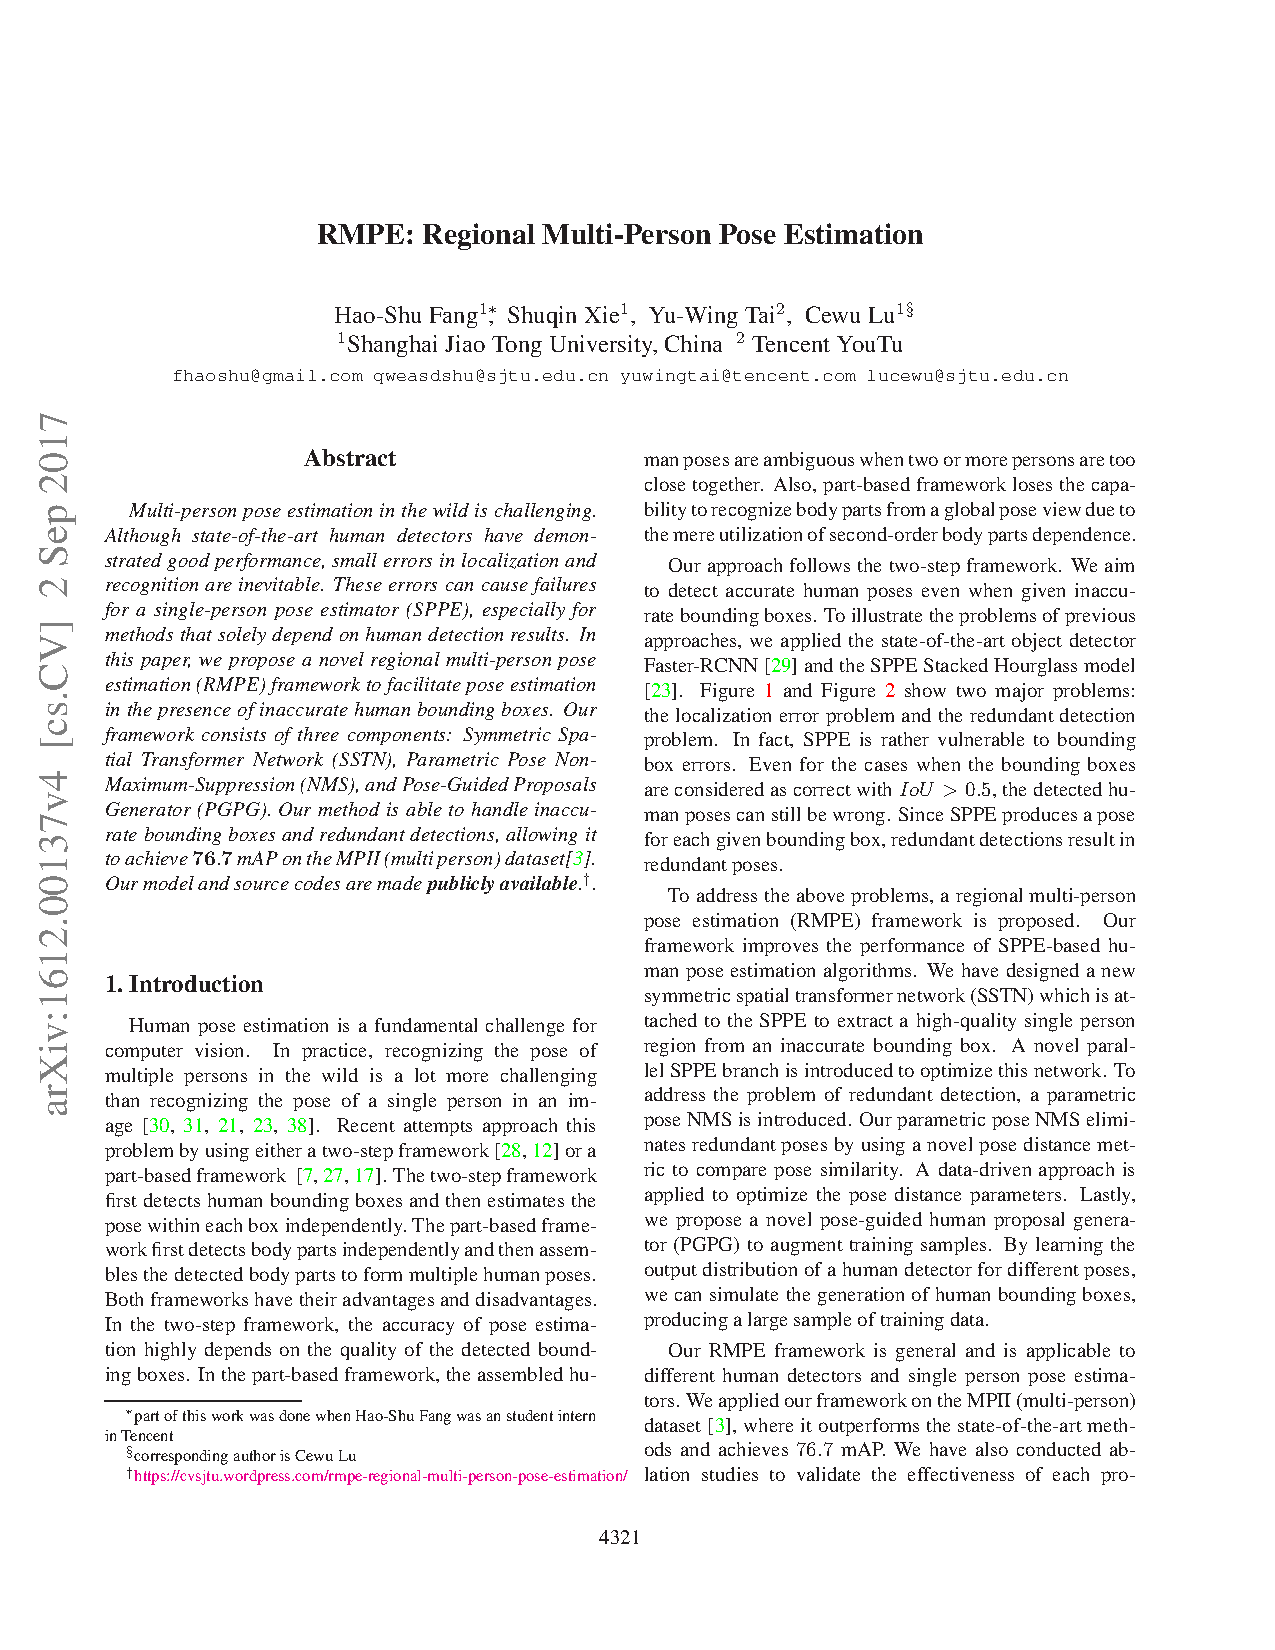
\includepdf[pages={1-}]{RMPE.pdf}